\documentclass[10pt]{article}
\usepackage{icmlko}

\icmlmeta{IP 파운데이션 월드모델}{132}{네 번째로 기제를 못 찾았다}{달력 축이 왜 도메인마다 갈리는지 --- 설명 넷을 세우고 넷 다 죽였다. 그런데 수치는 최고치를 갱신했다}

\begin{document}

\twocolumn[
\icmlheader

\begin{abstract}
노트 130에서 달력 축을 만든 뒤로 같은 질문이 남았다 --- \emph{왜 부스팅에서만
값을 하나.} 이번 노트는 그 답을 못 찾은 기록이다. \textbf{네 번째 설명까지
죽었다.} ① 부호가 도메인마다 갈려서(노트 130에서 검정, 틀림) ② 계수 방향
일치가 검색보다 낮아서(노트 131, 정황일 뿐) ③ 표본이 작은 도메인이
손해라서 --- \textbf{틀렸다}, $n$=25인 아이돌이 $+$0.082로 오르고 $n$=223인
게임이 $-$0.061로 내린다 ④ 도메인별 모수를 공유 계수가 눌러서 --- 그래서
\textbf{공유 몸통 $+$ 도메인별 달력 머리}를 지어 봤는데, 안쪽 분할 검정이
머리를 한 번도 안 샀고 강제로 달면 판 $\rho$가 $+$0.3902에서 $+$0.3796으로
\emph{단조롭게} 나빠진다. 거절이 옳았다. 그리고 ④를 죽이는 증거가 하나 더
있다. \textbf{TabPFN은 우리 자료로 모수를 정하지 않는데도 같은 벌점을
받는다} --- 검색으로 $+$0.3443에서 $+$0.3930으로 올랐다가 달력으로
$+$0.3721로 내린다. 모수가 원인이 아니라는 뜻이다. \textbf{그런데 수치는
올랐다.} 웹툰 덮음을 37.9\%에서 97.6\%로 채우자 부스팅이
\textbf{$+$0.4328}, 귀무 폭 \textbf{0.0591}, $z$ \textbf{$+$7.41}로 가드
여덟을 통과했다. 공통 다섯 축만 쓰던 $+$0.3363에서 $+$0.0965다. 마지막으로
\textbf{내 버그를 하나 잡았다} --- 학습에 못 든 도메인의 축 이름을 빠뜨려
팝업이 검색 축 없이 예측되고 있었고, 그 값($+$0.5601)이 진짜보다 높아서
이상하다고 판 것이 단서였다.
\end{abstract}
]

\begin{figure*}[t]
\centering
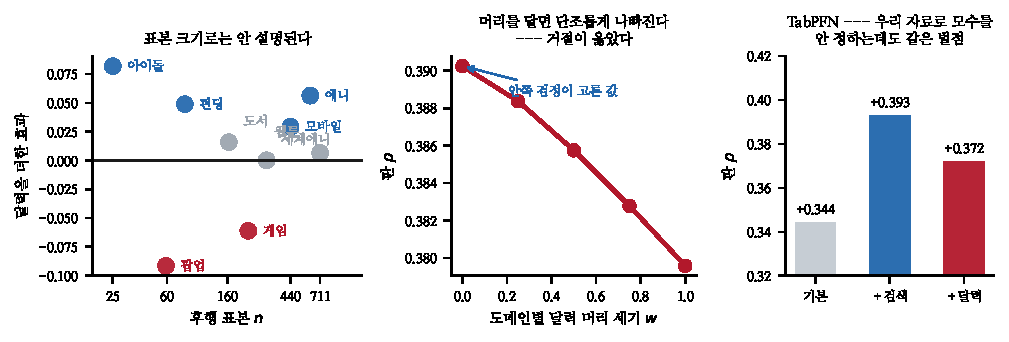
\includegraphics[width=\textwidth]{figs/hetero.pdf}
\caption{왼쪽 --- 달력 효과가 표본 크기로 설명되지 않는다. 가운데 ---
도메인별 달력 머리를 강제로 달면 단조롭게 나빠진다. 오른쪽 --- 우리 자료로
모수를 정하지 않는 TabPFN도 같은 벌점을 받는다.}
\end{figure*}

\section{먼저 오른 것}

웹툰 검색 축 덮음이 노트 129에서 할당량 소진으로 37.9\%에 멈춰 있었다.
채웠다 --- 97.6\%(2{,}750행), 전체 5{,}925행.

\begin{table}[t]
\centering\tsize
\caption{부스팅의 사다리. 가드 여덟 전부 통과.}
\begin{tabular}{lrrr}
\toprule
& 판 $\rho$ & 귀무 폭 & $z$ \\
\midrule
공통 다섯 & $+$.3363 & .0789 & $+$4.41 \\
$+$검색 (웹툰 38\%) & $+$.4107 & .0630 & $+$6.57 \\
$+$검색 $+$달력 (38\%) & $+$.4203 & .0579 & $+$7.31 \\
$+$검색 (웹툰 98\%) & $+$.4170 & .0665 & $+$6.35 \\
$+$검색 $+$달력 (98\%) & \textbf{$+$.4328} & .0591 & \textbf{$+$7.41} \\
\bottomrule
\end{tabular}
\end{table}

노트 125부터 정식화를 일곱 붙여 얻은 최대 폭이 $+$0.013이었고, 축 두 벌을
더한 이번 폭이 $+$0.0965다.

\section{그리고 못 찾은 것}

달력 축은 대상 아홉 중 일곱에서 오르고 둘에서 내린다.

\begin{table}[t]
\centering\tsize
\caption{달력을 더한 효과(부스팅). 후행 표본 순.}
\begin{tabular}{lrr}
\toprule
& $n$ & 효과 \\
\midrule
아이돌 & 25 & $+$.082 \\
\textbf{팝업} & 59 & \textbf{$-$.092} \\
펀딩 & 80 & $+$.049 \\
도서 & 163 & $+$.016 \\
\textbf{게임} & 223 & \textbf{$-$.061} \\
세계애니 & 300 & $+$.000 \\
모바일 & 441 & $+$.029 \\
애니 & 606 & $+$.056 \\
웹툰 & 711 & $+$.007 \\
\bottomrule
\end{tabular}
\end{table}

\claimx{\textbf{표본 크기가 기제가 아니다.} 제일 작은 아이돌($n$=25)이
$+$0.082로 오르고 게임($n$=223)이 $-$0.061로 내린다. 지는 것은 팝업과 게임
둘뿐이고, 둘을 묶는 성질을 아직 못 찾았다.}{처음에 ``작은 도메인이
손해''라고 읽었다. 표를 표본 순으로 세워 보고서야 아니라는 것을 알았다 ---
\textbf{정렬을 바꿨을 뿐인데 결론이 바뀌었다.}}

이 기제를 찾으려고 세운 설명이 넷이고 넷 다 죽었다.

\begin{table}[t]
\centering\tsize
\caption{죽은 설명 넷.}
\begin{tabular}{lll}
\toprule
& 설명 & 어떻게 죽었나 \\
\midrule
① & 한계 부호가 갈려서 & 일치하는 것만 쓰면 더 낮다 \\
② & 계수 방향이 덜 공유돼서 & 정황($+$.198 대 $+$.331) \\
③ & 표본이 작은 쪽이 손해 & 아이돌 $n$=25가 오른다 \\
④ & 공유 계수가 눌러서 & 머리를 달면 나빠진다 \\
\bottomrule
\end{tabular}
\end{table}

\subsection{④를 죽인 두 증거}

넷째가 제일 그럴듯했다. 달력 관계가 도메인마다 다르니 공유 계수 하나로는
못 담고, 트리는 도메인 표시자로 쪼갤 수 있어서 되는 것이라면 ---
\textbf{쪼개 주면} 선형에서도 돼야 한다. 그래서 지었다.

축과 검색은 전 도메인이 함께 배우고(몸통), 달력만 도메인마다 잔차를
고친다(머리). 머리 세기 $w_d$ 는 노트 126의 교훈대로 학습 기간 안쪽
분할로만 정한다.

\claimx{\textbf{안쪽 검정이 머리를 한 번도 안 샀고, 그 거절이 옳았다.}
아홉 도메인 전부 $w_d$=0이 나왔다. 강제로 달아 보니 판 $\rho$가 $w$=0에서
$+$0.3902, 0.25에서 $+$0.3884, 0.5에서 $+$0.3857, 1.0에서 $+$0.3796으로
\emph{단조롭게} 내린다.}{팝업은 머리 자체가 없다 --- 2025년 이전 레코드가
16건이라 학습 도메인에 못 든다. 노트 131의 팝업 $+$0.513은 시간을 안 가른
무작위 교차검증 값이고, 배포 규약으로는 재현할 수가 없다.}

두 번째 증거가 더 세다.

\claimx{\textbf{TabPFN도 같은 벌점을 받는다.} 표 자료 사전학습 트랜스포머는
우리 자료로 모수를 정하지 않고 학습 표를 문맥에 넣어 한 번 통과시킨다.
그런데 검색으로 $+$0.3443에서 $+$0.3930으로 올랐다가 달력으로 $+$0.3721로
내린다 --- 부스팅 말고는 다 같은 모양이다. \textbf{그러니 원인은 우리가
정하는 모수가 아니다.}}{TabPFN 문맥을 3{,}000행으로 잘랐다. 문맥이 길면
달라질 수 있다.}

남는 것은 관측이다. \textbf{달력 축은 부스팅에서만 값을 하고, 왜인지는
아직 모른다.} 네 번 틀린 뒤에는 다섯째 설명을 세우기보다 이렇게 적어 두는
것이 맞다고 본다.

\section{잡은 버그}

F16을 처음 돌렸을 때 팝업이 $+$0.5601로 나왔다. 몸통이 F9와 같은 자료·같은
축인데 F9의 팝업은 $+$0.5101이다. \textbf{계수를 찍어 보니 완전히 같은데
예측 상관이 0.923이었다} --- 같은 모형이 다른 입력을 보고 있다는 뜻이다.

\claimx{\textbf{학습에 못 든 도메인의 축 이름을 빠뜨렸다.} 몸통에 줄 자료를
만들면서 달력 열을 뺄 때 \texttt{data.dom} 만 돌았는데, 팝업은 2025년 이전
16건이라 \texttt{dom} 에 없다. 그래서 팝업의 축 이름이 사라지고 자질
생성기가 기본 다섯으로 되돌아가 \textbf{팝업이 검색 축 없이 예측되고
있었다.}}{그 값이 진짜보다 \emph{높았다}는 것이 단서였다 --- 팝업은 검색
축을 빼는 게 낫다는 것을 노트 128부터 세 번 봤으니까. 수치가 이상한 게
아니라 \emph{방향이 알던 것과 맞아떨어져서} 의심했다.}

\section{남은 것}

\begin{table}[t]
\centering\tsize
\caption{다음.}
\begin{tabular}{ll}
\toprule
팝업 & 2025년 이전 16건이 배포 규약의 병목이다 \\
달력 & 기제를 다섯 번째로 찾지 않는다. 관측으로 둔다 \\
모바일 · 게임 & 제목 언어로 덮음이 30$\sim$41\%에 묶여 있다 \\
\bottomrule
\end{tabular}
\end{table}

팝업이 두 갈래에서 같은 벽에 닿았다. 노트 131의 ``무엇을 $+$ 언제''
$+$0.513은 무작위 교차검증이라 시간을 안 가르고, 배포 규약으로 옮기면
학습에 쓸 팝업이 16건뿐이라 머리를 달 수가 없다. \textbf{팝업의 병목은
모형도 축도 아니라 2025년 이전 표본이다.} 노트 124가 열고 노트 127이
좁힌 그 길이 다시 제일 큰 한 수다.

\end{document}
